\subsubsection{To add a question:}

\begin{figure}[H]
	\begin{subfigure}{0.70\linewidth}
		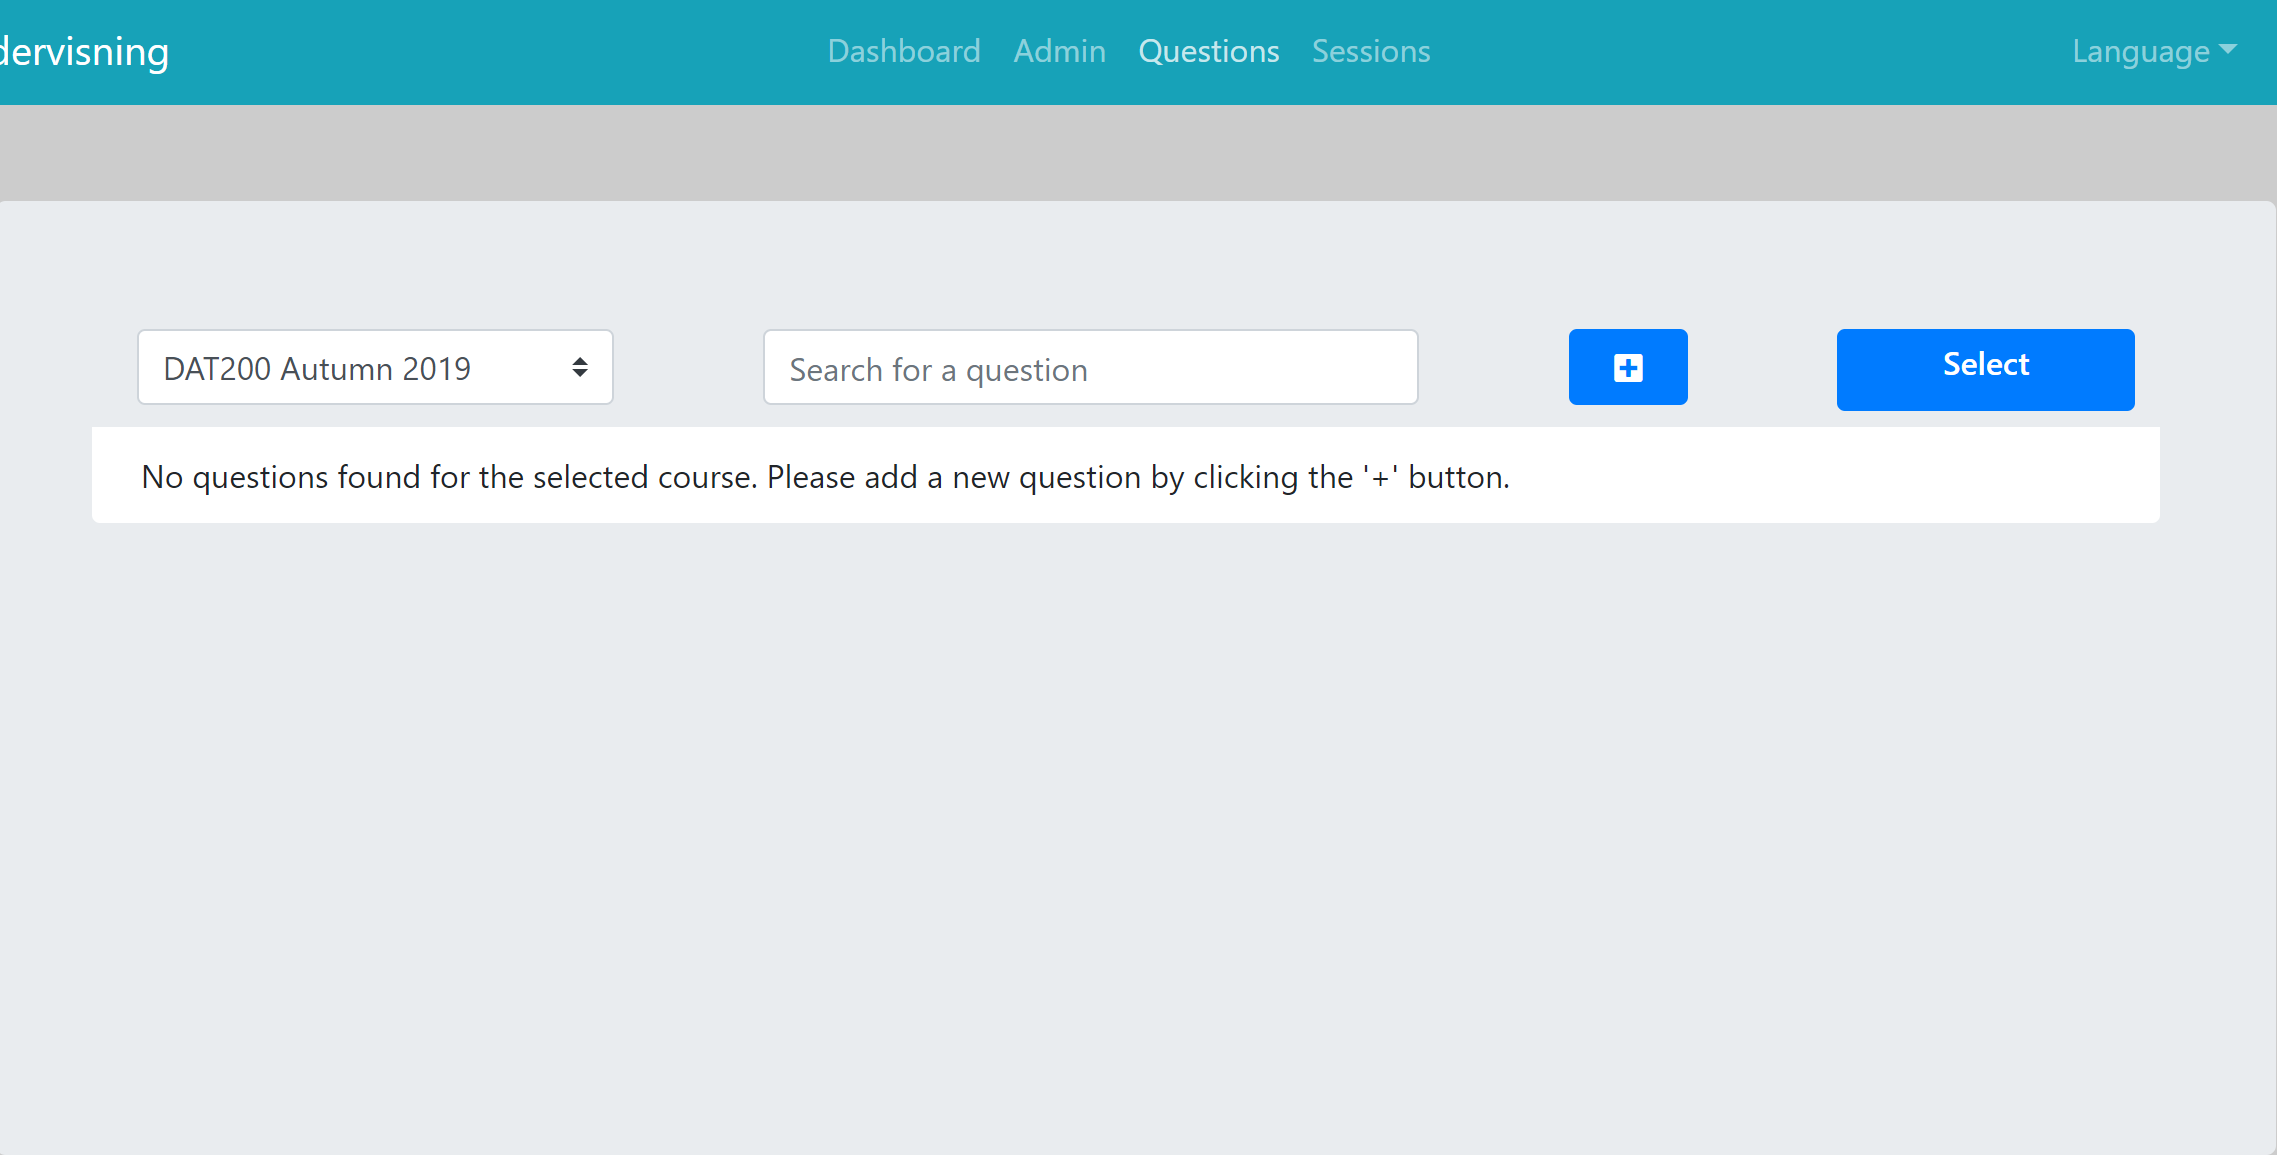
\includegraphics[width=\linewidth]{userManual/admin/QuestionDashboardEmpty}
		\caption{}
		\label{fig:QuestionDashboardEmpty}
	\end{subfigure}
	\begin{subfigure}{0.70\linewidth}
		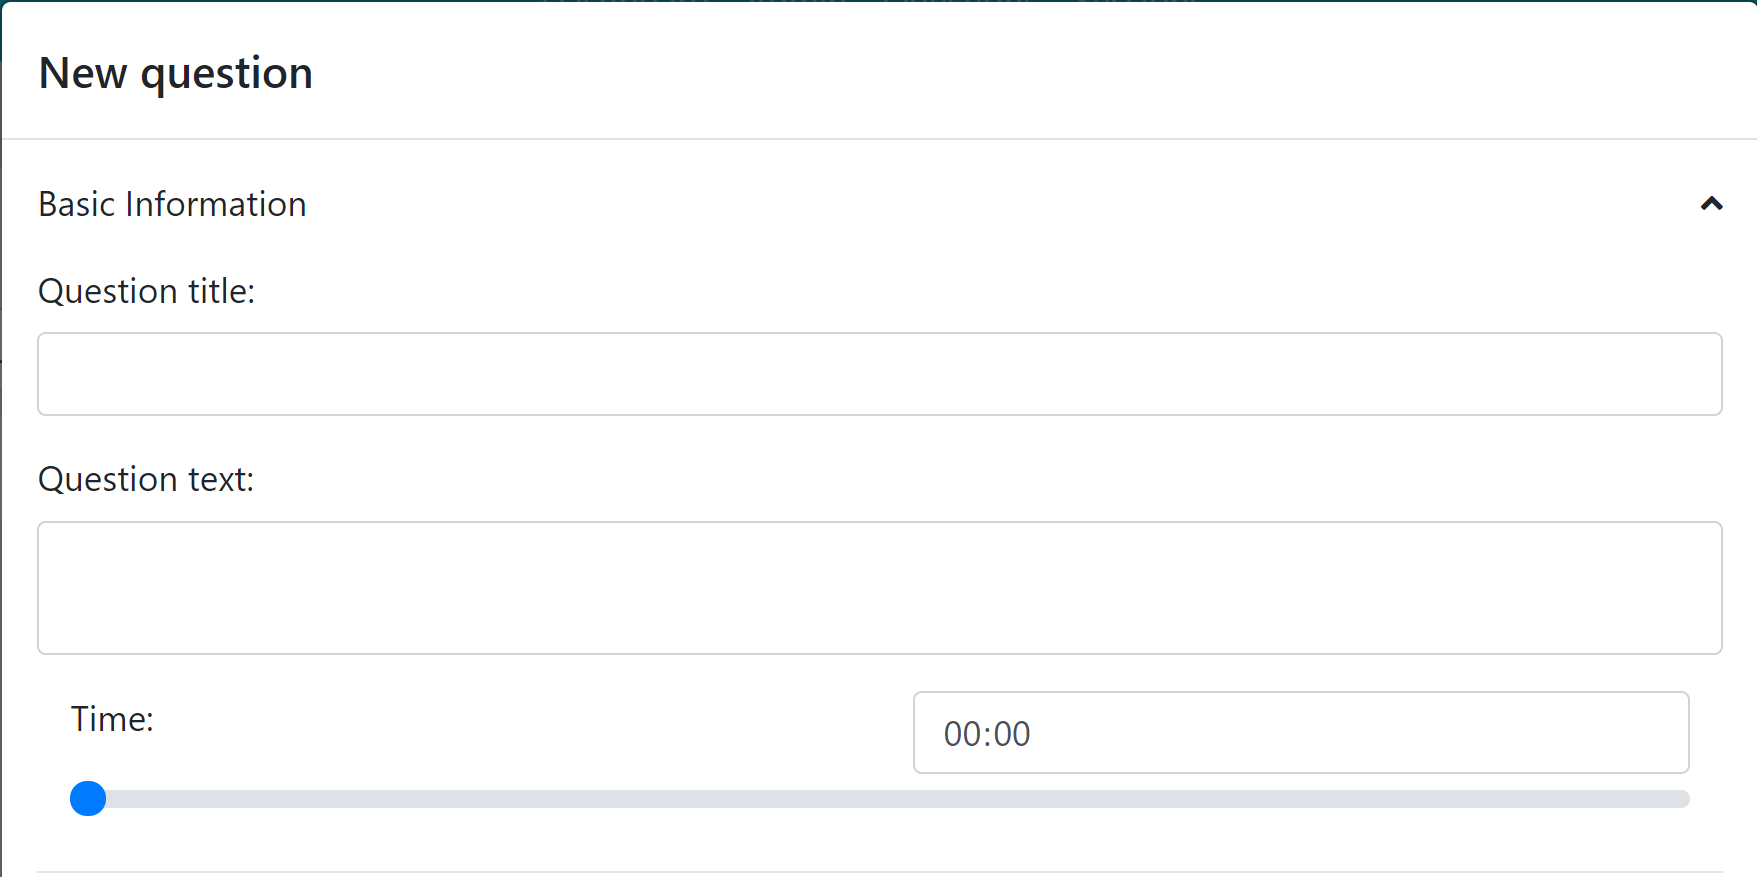
\includegraphics[width=\linewidth]{userManual/admin/EditQuestionBasicInfo}
		\caption{}
		\label{fig:EditQuestionBasicInformation}
    \end{subfigure}
	\begin{subfigure}{0.70\linewidth}
		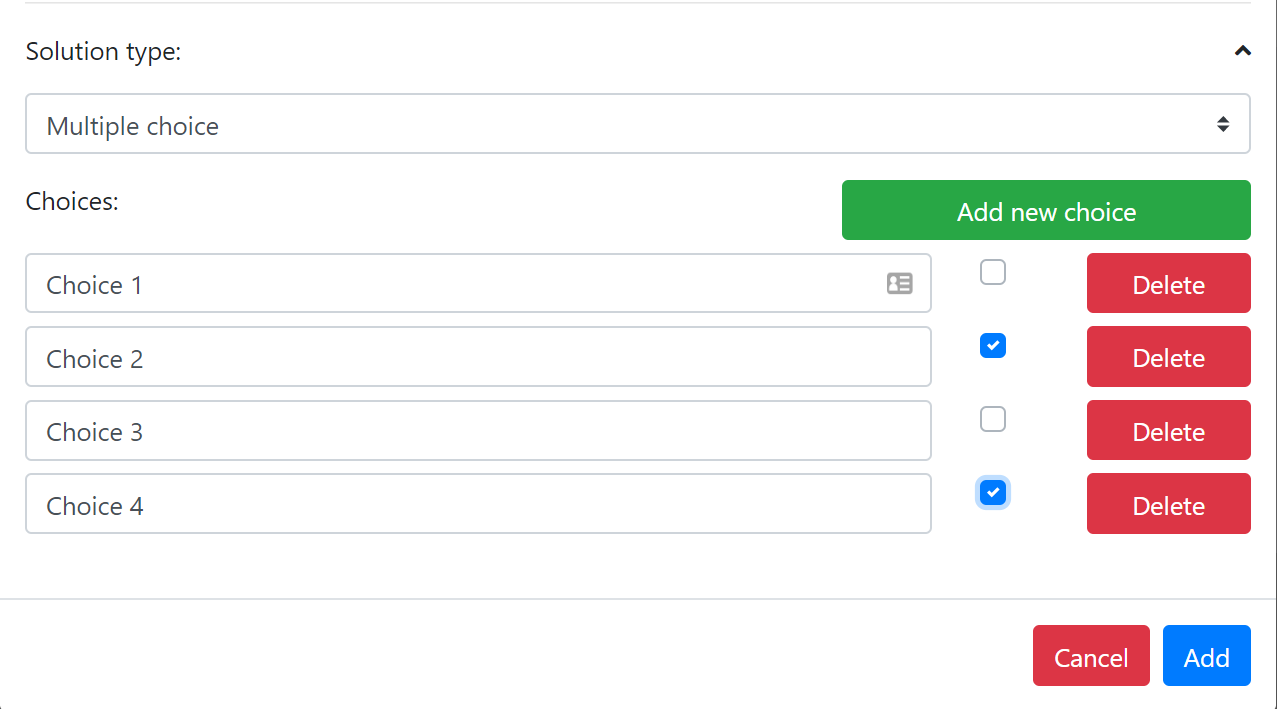
\includegraphics[width=\linewidth]{userManual/admin/EditQuestionSolution}
		\caption{}
		\label{fig:EditQuestionSolution}
	\end{subfigure}
\end{figure}

\begin{userManualItemlist}
    \item[Step I.] Navigate to the questions page.
    \item[Step II.] Click the "+" button. (Figure: \ref{fig:QuestionDashboardEmpty})
    \item[Step III.] Enter the question information in the title and description fields. (Figure: \ref{fig:EditQuestionBasicInformation})
    \item[Step IV.] If you want a timed question, select the time with the slider or the input field. (Figure: \ref{fig:EditQuestionBasicInformation})
    \item[Step V.] If you want to add media to a question see the section for adding media to a question.
    \item[Step VI.] Click "Solution type". (Figure: \ref{fig:EditQuestionSolution})
    \item[Step VII.] Select the solution type from the select element. (Figure: \ref{fig:EditQuestionSolution})
    \item[Step VIII.] Follow the instructions on the screen to enter the required information. (Figure: \ref{fig:EditQuestionSolution})
    \item[Step IX.] Click the "Add" button. 
\end{userManualItemlist}

\subsubsection{To edit a question:}
\begin{userManualItemlist}
    \item[Step I.] Navigate to the questions page.
    \item[Step II.] Click the edit (pen and paper symbol) button.
    \item[Step III.] Edit the information.
    \item[Step IV.] Click the "Add" button.  
\end{userManualItemlist}

\subsubsection{To add media to a question:}

\begin{figure}[H]
	\begin{subfigure}{0.70\linewidth}
		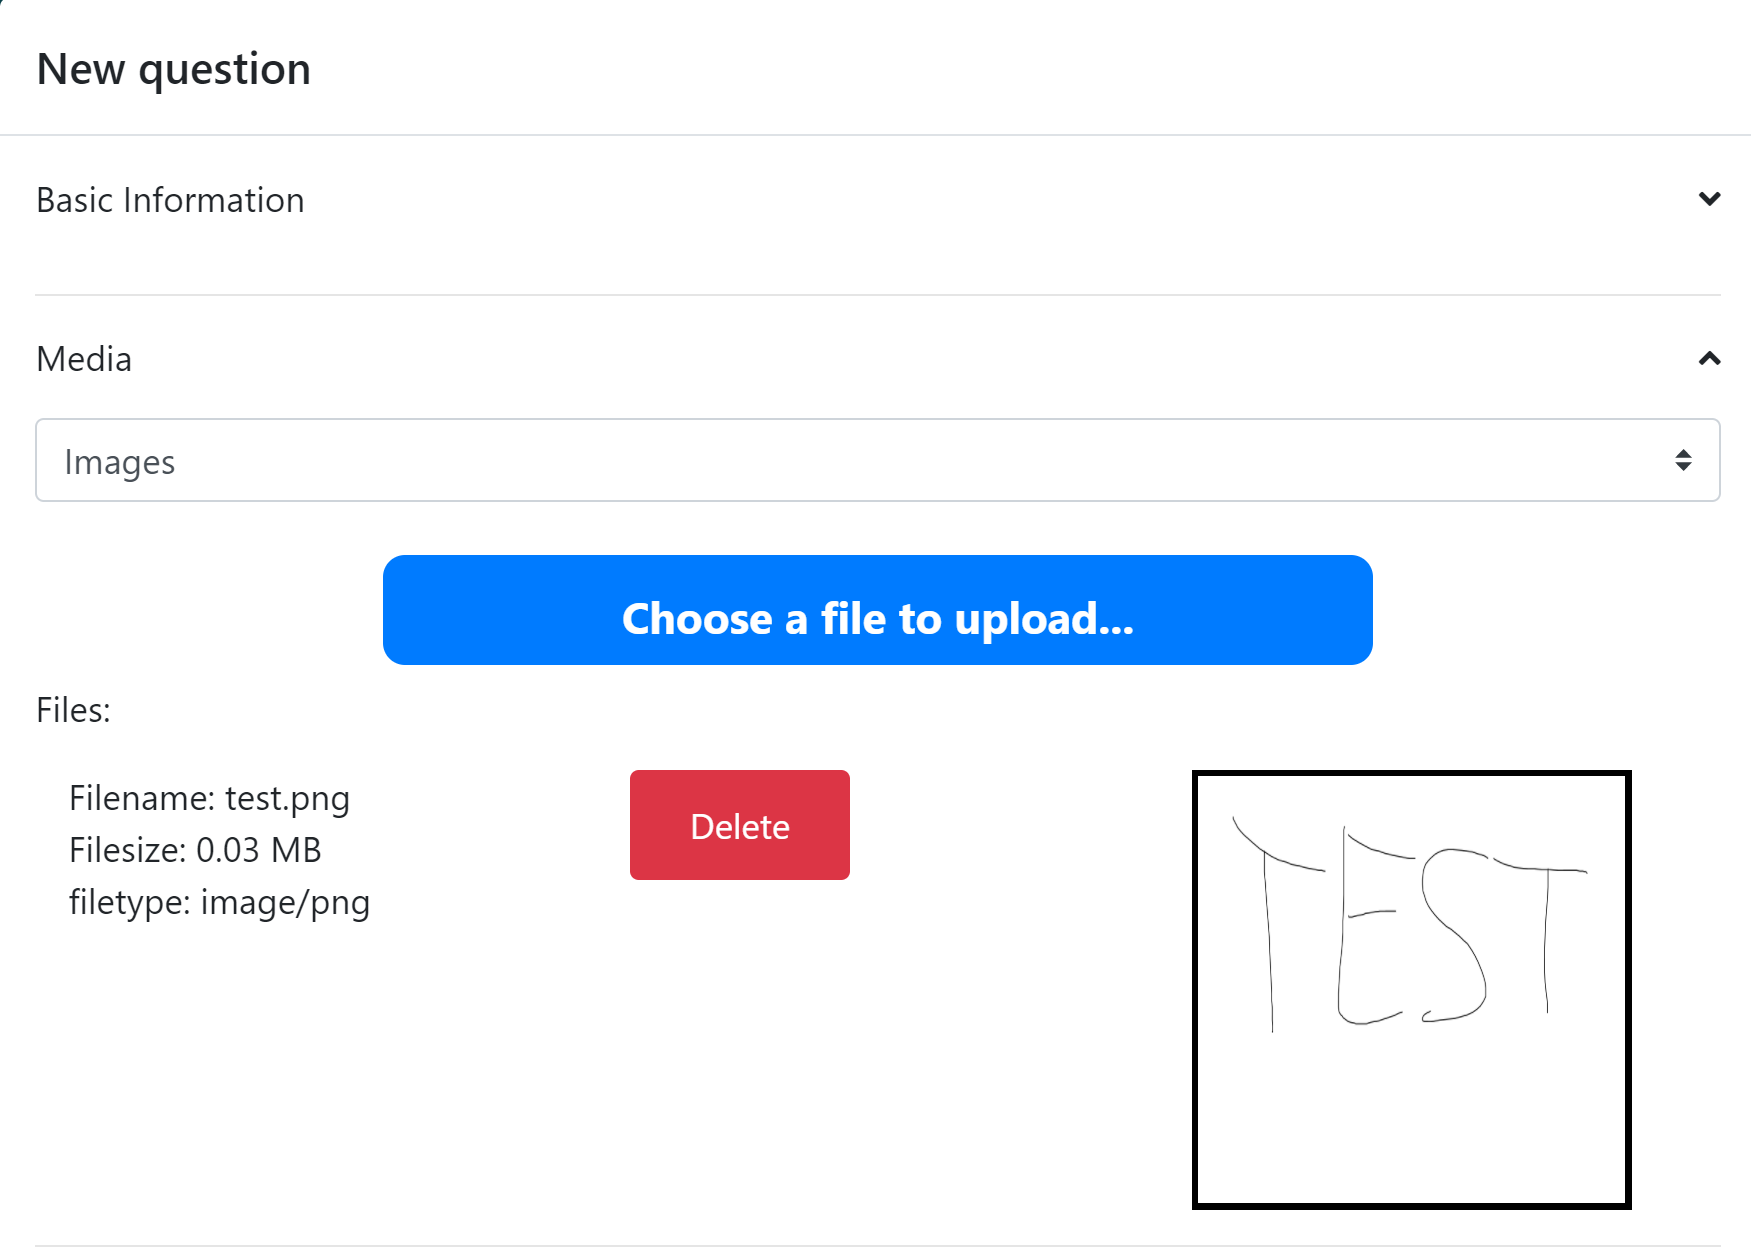
\includegraphics[width=\linewidth]{userManual/admin/EditQuestionImageMediaPNG}
		\caption{}
		\label{fig:EditQuestionImageMedia}
	\end{subfigure}
	\begin{subfigure}{0.70\linewidth}
		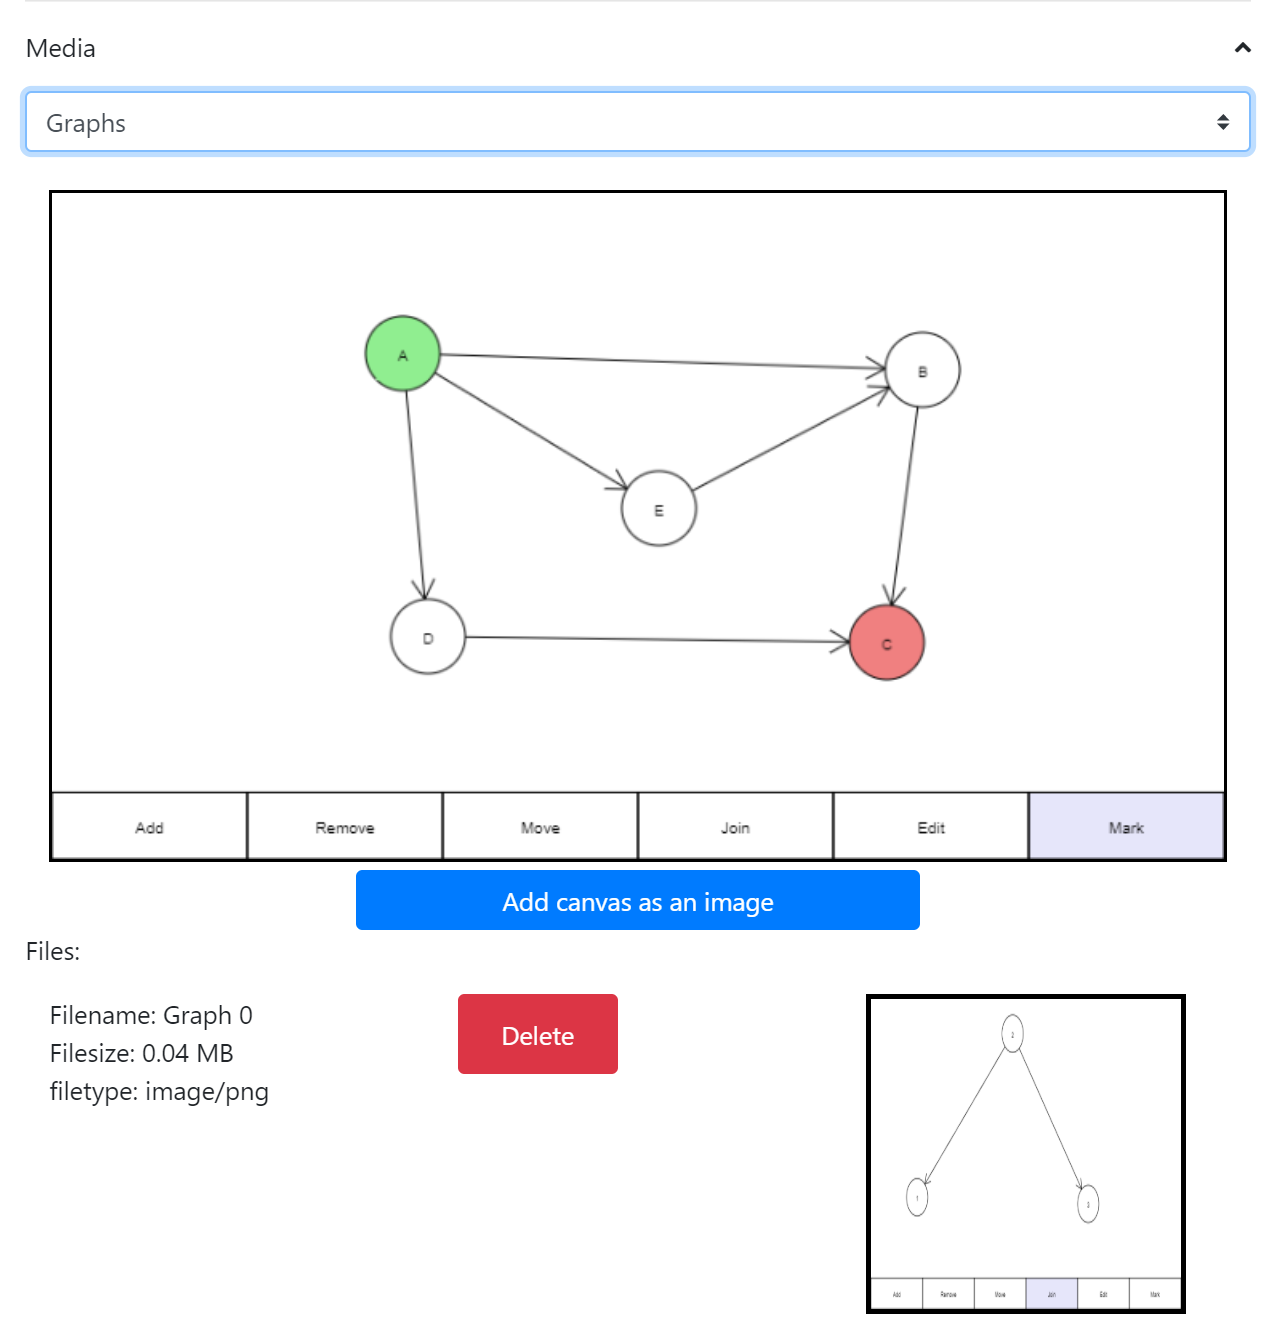
\includegraphics[width=\linewidth]{userManual/admin/EditQuestionGraphMedia}
		\caption{}
		\label{fig:EditQuestionGraphMedia}
    \end{subfigure}
	\begin{subfigure}{0.70\linewidth}
		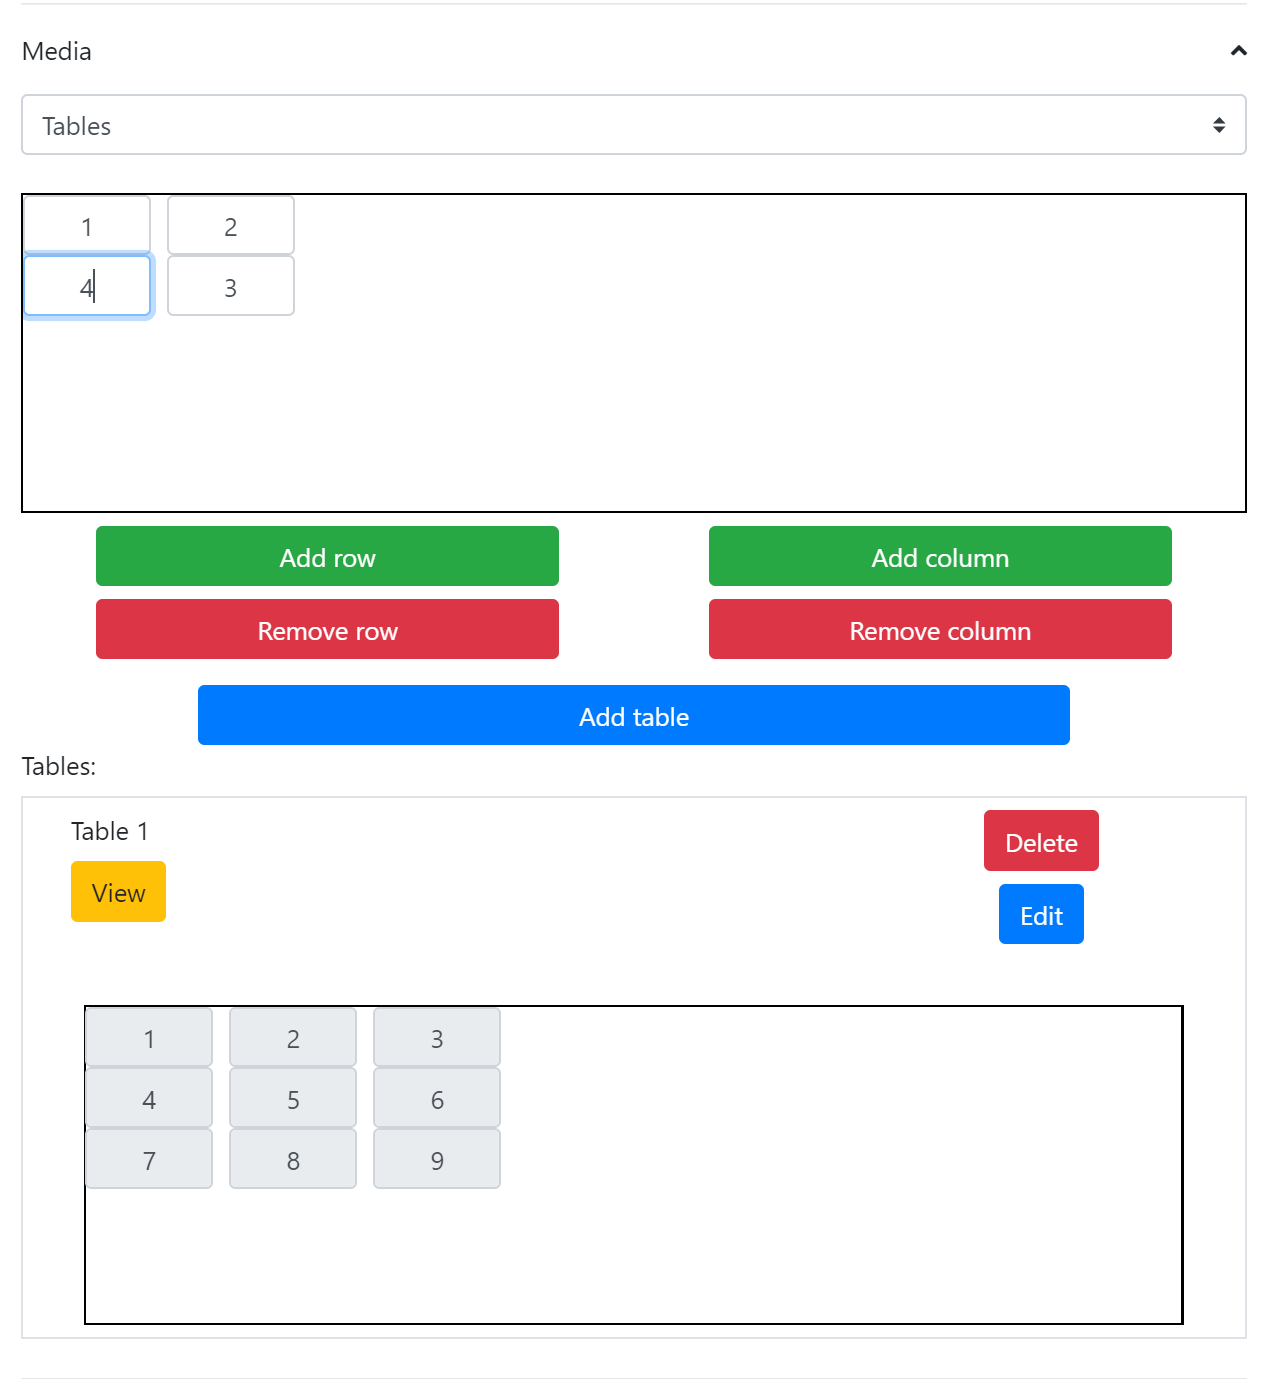
\includegraphics[width=\linewidth]{userManual/admin/EditQuestionTablesMedia}
		\caption{}
		\label{fig:EditQuestionTableMedia}
	\end{subfigure}
\end{figure}

\begin{userManualItemlist}
    \item[Step I.] Click "Media".
    \item[Step II.] Select what type of media you want to include.
    \item[Step III.] If you are adding images, click the "Choose a file to upload..." button. This will open a file browser where you can select the images. (Figure: \ref{fig:EditQuestionImageMedia})
    \item[Step IV.] If you added an image by mistake, it can be removed by clicking the "Delete" button. (Figure: \ref{fig:EditQuestionImageMedia})
    \item[Step V.] If you are adding a graph, use the GraphDrawer tool to create it. (Figure: \ref{fig:EditQuestionGraphMedia})
    \item[Step VI.] When you are done, click the "Add canvas as image" button. (Figure: \ref{fig:EditQuestionGraphMedia})
    \item[Step VII.] If you are adding a table, use the add and remove buttons to create the table. (Figure: \ref{fig:EditQuestionTableMedia})
    \item[Step VIII.] Click on table cells to enter the value. (Figure: \ref{fig:EditQuestionTableMedia})
    \item[Step IX.] When you are done, click the "Add table" button. (Figure: \ref{fig:EditQuestionTableMedia})
\end{userManualItemlist}
